\section{Chaotic Encryption:  Sound Bytes}
    
    \frame{\sectionpage}
    
    \begin{frame}
        \centering
        What if you could encrypt real-time?
    \end{frame}
    
    \begin{frame}{Creating a Physical Key}
        \centering
        Components:
        \begin{itemize}
        	\item A message:  $a$ $sound$ $byte$
        	\item A method to encode:  $masking$ $with$ $static$
        	\item A method to decode:  $filtering$ $out$ $static$
        	\item A key:  $coupled$ $systems$
        \end{itemize}
    \end{frame}     
    
    \begin{frame}{The Theory of Coupled Systems}
        \begin{minipage}[b]{0.45\linewidth}
            \centering
            \caption{Master System}
            \label{lst}
            \begin{equation*}
                \begin{cases} 
                    \dot{x_{m}} = \sigma(y-x) \\ 
                    \dot{y_{m}} = rx - y - xz \\ 
                    \dot{z_{m}} = xy - bz
                \end{cases}
            \end{equation*}
        \end{minipage}
        \hspace{0.5cm}
        \begin{minipage}[b]{0.45\linewidth}
            \centering
            \caption{Receiver System}
            \label{lst}
            \begin{equation*}
                \begin{cases} 
                    \dot{y_{r}} = rx - y_{r} - xz_{r} \\ 
                    \dot{z_{r}} = xy_{r} - bz_{r}
                \end{cases}
            \end{equation*}
        \end{minipage}
    \end{frame}
    
    \begin{frame}{A Physical Coupled System}
        \begin{figure}
            \centering
            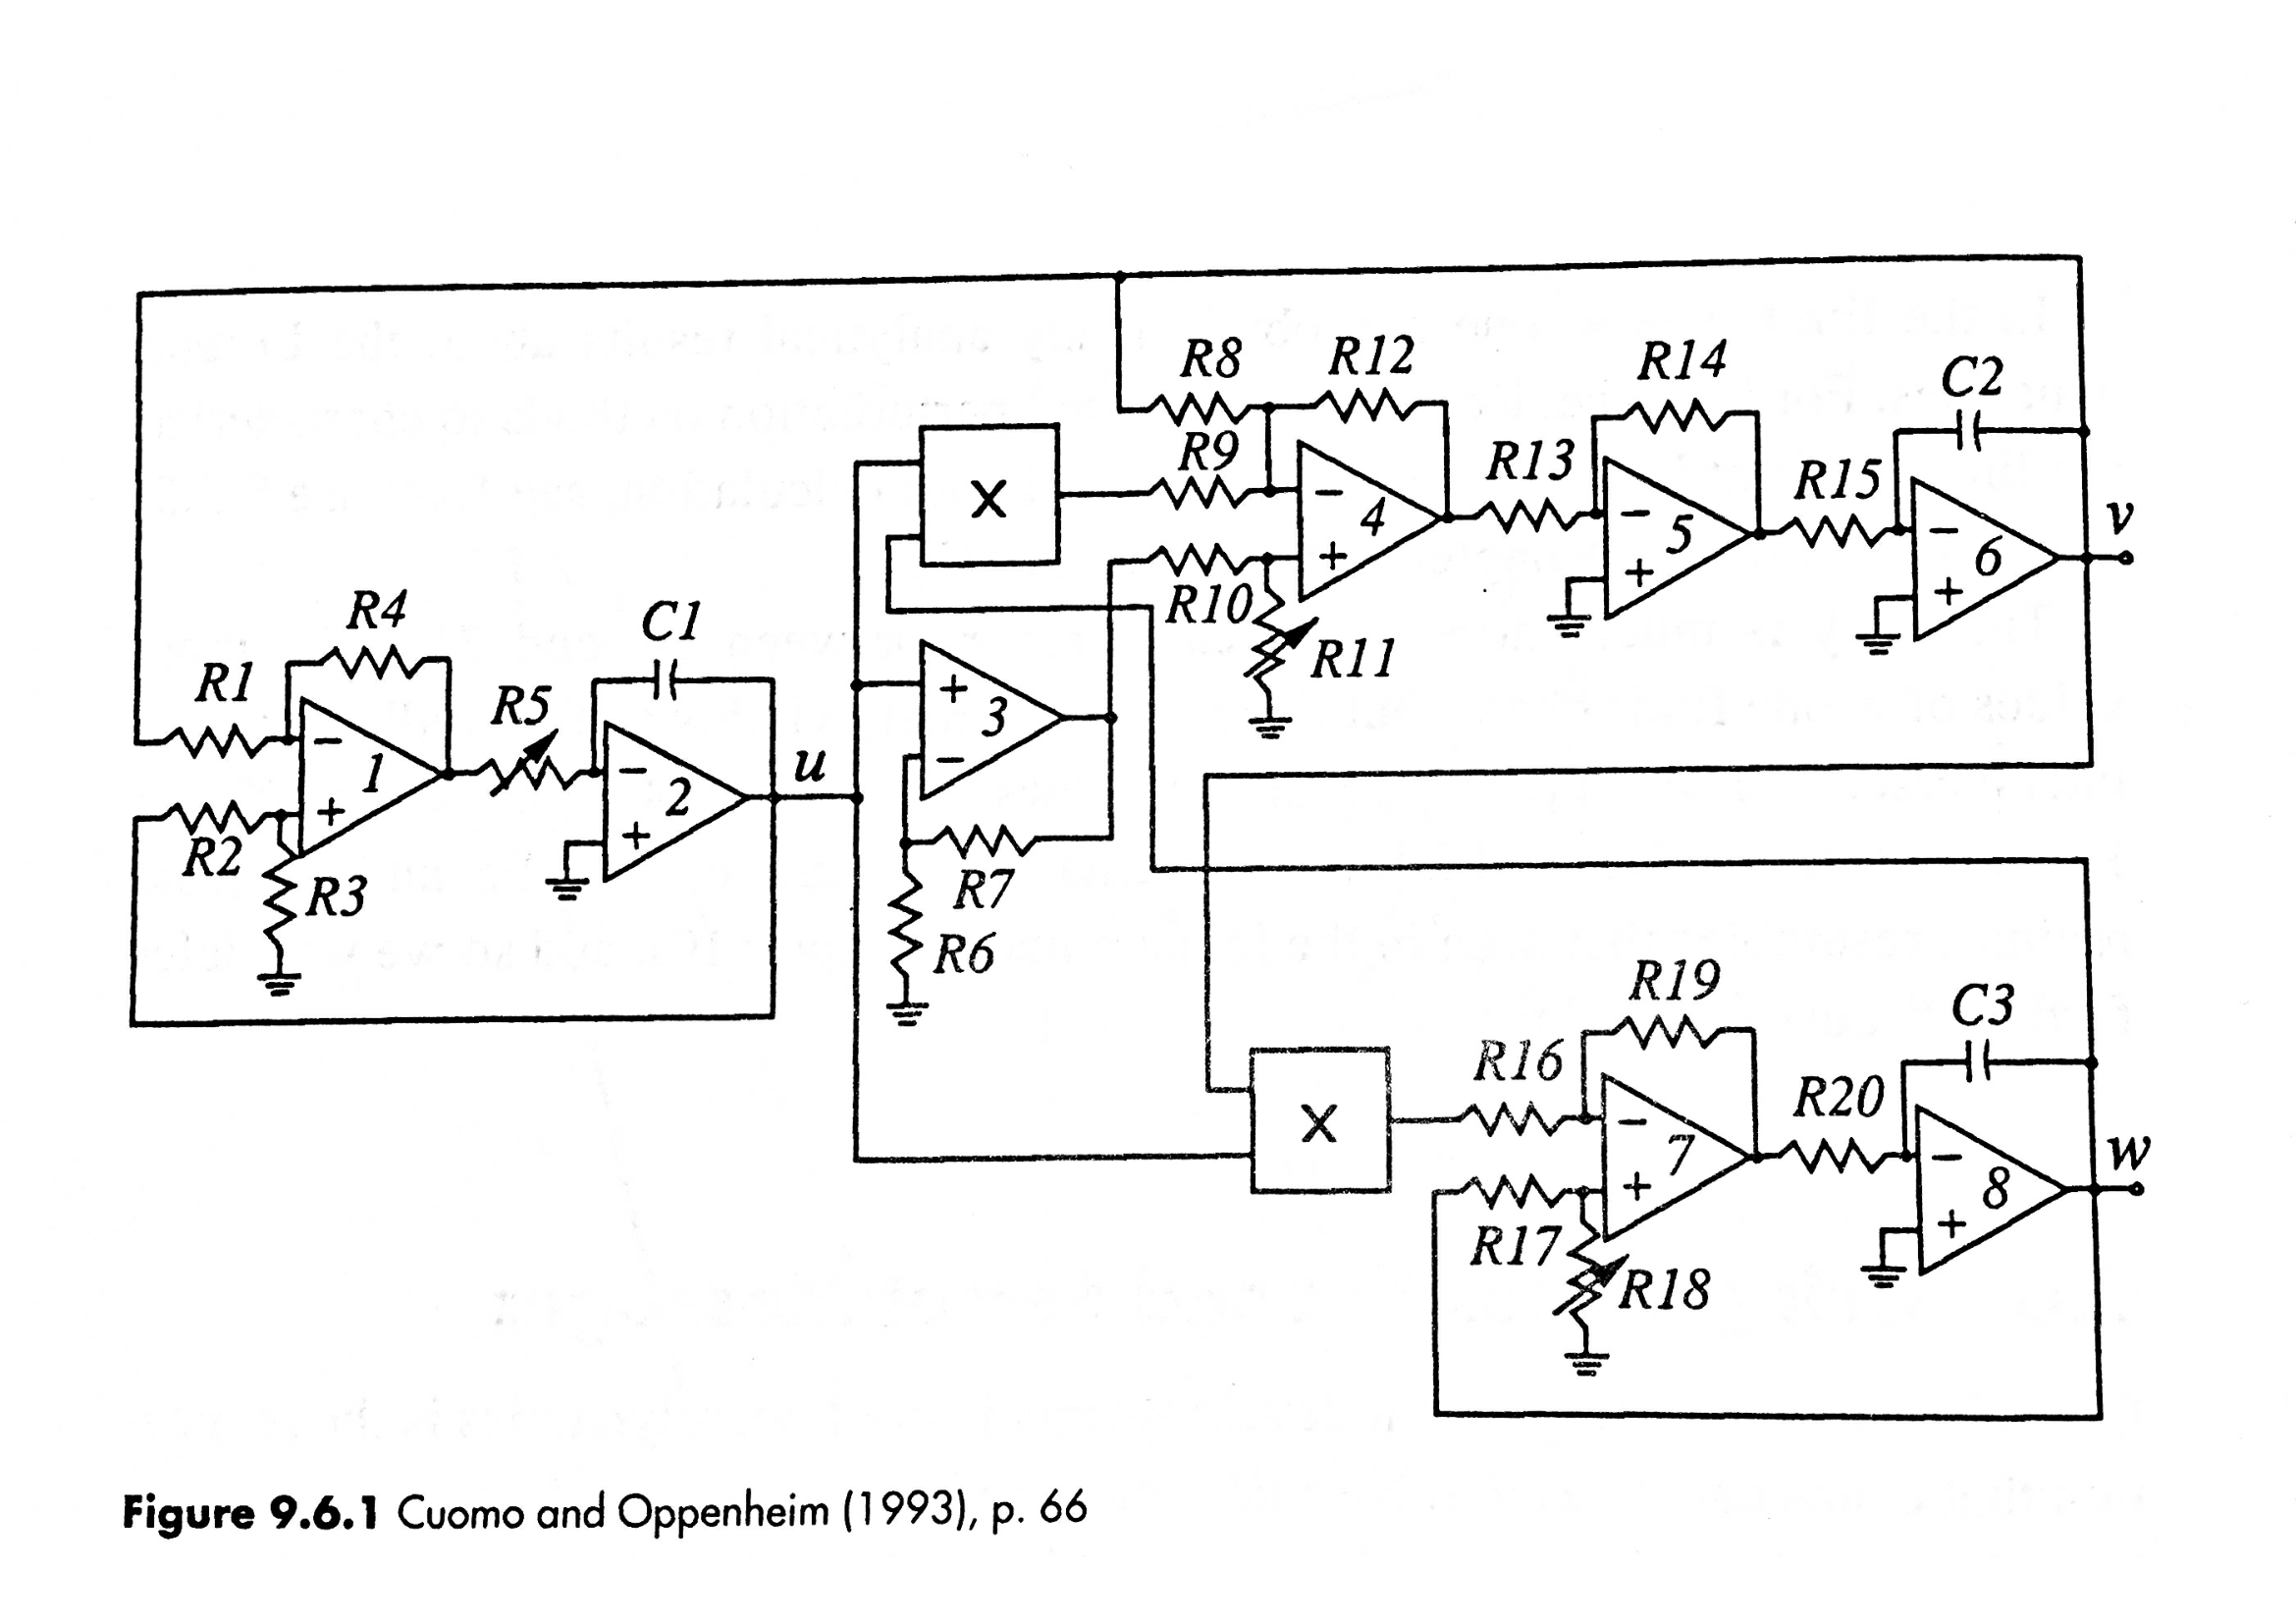
\includegraphics[height=5cm]{circuit.png}
            \caption{this RC circuit is one half of a coupled system}
            \label{fig}
        \end{figure}
    \end{frame}
